\documentclass{article}
\usepackage{cmap}
\usepackage[T2A]{fontenc}
\usepackage[utf8]{inputenc}
\usepackage[english,russian]{babel}
\usepackage{setspace}
\usepackage{geometry}
\usepackage{graphicx}
\usepackage{amsfonts}
\graphicspath{{graphicslab2/}}
\DeclareGraphicsExtensions{.pdf, .png, .jpg, .fig}
\geometry{top=2cm}
\geometry{bottom=2cm}
\geometry{left=2cm} % отступ справа
\geometry{right=2cm} % отступ слева

\begin{document}
	\begin{center}
		\hfill \break
		\begin{center}
			\huge{Санкт-Петербургский политехнический университет\\
				Высшая школа прикладной математики\\
				и вычислительной физики, ФизМех}
		\end{center}
		\hfill \break
		\hfill \break
		\hfill \break
		\hfill \break
		\hfill \break
		\huge{Направление подготовки\\
			«Прикладная математика и информатика»}\\
		\hfill \break
		\hfill \break
		\hfill \break
		\hfill \break
		\hfill \break
		\hfill \break
		\fontsize{14pt}{14pt}\selectfont
		Отчет по лабораторной работе №2\\
		«Решение СЛАУ прямыми методами»\\
		\hfill \break
		\hfill \break
		\hfill \break
		\hfill \break
		\hfill \break
	\end{center}
	\hfill \break
	\hfill \break
	\fontsize{12pt}{12pt}\selectfont
	\begin{tabular}{cccc}
		\hspace{1cm}Выполнил студент гр. 5030102/00003 & {\hspace{3cm}} & & Петрошенко А.В. \\\\
		\hspace{-3cm}Преподаватель: &{\hspace{1cm}}& & {\hspace{1cm}} Курц В.В. \\\\
	\end{tabular}\\
	\hfill \break
	\hfill \break
	\hfill \break
	\hfill \break
	\hfill \break
	\hfill \break
	\begin{center} Санкт-Петербург\\ 
		2021\\
	\end{center}
	\thispagestyle{empty}
	\newpage
	\begin{center} \textbf{Формулировка задачи и ее формализация}\end{center}
	Большинство расчетных математических задач сводится к решению системы линейных алгебраических уравнений(далее СЛАУ). Существует 2 класса методов решения таких СЛАУ:
	\begin{enumerate}
		\item Прямые методы - методы, которые находят <<точные>> значения неизвестных за конечное число операций.
		\item Итерационные методы - методы, которые строят последовательность векторов, сходящихся к решению.
	\end{enumerate}
	В этой работе мы будем использовать прямой метод.\\
	\\
	\underline{Постановка задачи:}\\
	Пусть дана система из $n$ линейных уравнений с $n$ неизвестными:
	\begin{center}
		$\sum\limits_{j = 1}^n a_{ij}x_j = b_i$, $i = 1, \ldots, n$
	\end{center}
	где $x_j$ - неизвестные, $a_{ij}$ - коэффициенты системы и $b_i$ - компоненты вектора правой части.\\
	В матричной форме:
	\begin{center}
		$Ax = b$
	\end{center}
	где $A = (a_{ij}) \in \mathbb{R} ^{n \times n}$ - матрица коэффициентов, $b = (b_i) \in \mathbb{R}^n$ - вектор правой части и $x = (x_j) \in \mathbb{R}^n$ - вектор неизвестных.\\
	Требуется найти $x$, решив СЛАУ методом Холецкого и исследовать вычислительную ошибку для матриц с разными числами обусловленности.
	\begin{center} \textbf{Алгоритм метода и условия его применимости}\end{center}
	Пусть $A \in \mathbb{R}^{n \times n}$ - симметричная и положительно определенная матрица. Тогда $\exists!\ S:\ A = SS^T$, где $S$ - нижняя треугольная матрица.\\
	$S = \left(
	\begin{array}{cccc}
		s_{11} & 0 & \ldots & 0\\
		s_{21} & s_{22} & \ldots & 0\\
		\vdots & \vdots & \ddots & \vdots\\
		s_{n1} & s_{n2} & \ldots & s_{nn}
	\end{array}
	\right)$\\
	Подставляя в матричную форму СЛАУ, получаем:\\
	$Ax = b \Leftrightarrow S(S^Tx) = b \Leftrightarrow \left\{
	\begin{array}{lr}
	Sy = b\\
	S^Tx = y
	\end{array}
	\right.$
	\\
	\underline{Алгоритм метода Холецкого:}
	\begin{center}$A = SS^T \Leftrightarrow a_{ij} = \sum\limits_{k = 1}^n s_{ik}s_{kj}^T = \sum\limits_{k = 1}^n s_{ik}s_{jk}$\end{center}
	\textbf{Шаг 1.} $a_{11} = s_{11}^2 + \underbrace{s_{12}^2 + \ldots}_{=0} \Rightarrow s_{11} = \sqrt{a_{11}}$\\
	\hspace*{1.5 cm} $j > 1$: $a_{1j} = s_{11}s_{j1} + \underbrace{s_{12}s_{j2} + \ldots}_{=0} \Rightarrow s_{j1} = \frac{a_{1j}}{s_{11}}$\\
	<$\ldots$>\\
	\textbf{Шаг m.} $a_{mm} = \sum\limits_{k=1}^{m-1}s_{mk}^2 + s_{mm}^2 + \underbrace{\sum\limits_{k=m+1}^n s_{mk}^2}_{=0} \Rightarrow s_{mm} = \sqrt{a_{mm} - \sum\limits_{k = 1}^{m-1}s_{mk}^2}$\\
	\hspace*{1.5 cm} $j > m$: $a_{mj} = \sum\limits_{k=1}^{m-1}s_{mk}s_{jk} + s_{mm}s_{jm} + \underbrace{\sum\limits_{k=m+1}^{n}s_{mk}s{jk}}_{=0} \Rightarrow s_{jm} = \frac{a_{mj} - \sum\limits_{k=1}^{m-1}s_{mk}s_{jk}}{s_{mm}}$
	\newpage
	\hspace*{-0.65 cm} \underline{Условия применимости:}\\
	Квадратная матрица $A$ должна быть симметричной и положительно определенной.
	\begin{center} \textbf{Предварительный анализ задачи}\end{center}
	\underline{Построение матрицы:}\\
	Любую симметричную матрицу можно разложить в виде $A = QDQ^T$, где матрица $Q$ - это ортогональная матрица, а $D$ - диагональная матрица, на диагонали которой стоят только положительные числа. Т.к. они являются собственными числами матрицы $A$, то из данного разложения следует, что она будет и положительно определенной.
	\begin{center} \textbf{Тестовый пример для задач малой размерности}\end{center}
	Рассмотрим следующую СЛАУ:
	$\left\{
	\begin{array}{ccc}
		4x_1 + 2x_2 + 3x_3 = 4\\
		2x_1 + 2x_2 + 3x_3 = -5\\
		3x_1 + 3x_2 + 5x_3 = 6
	\end{array}
	\right.$\\
	Матрица $A = \left(
	\begin{array}{ccc}
		4 & 2 & 3\\
		2 & 2 & 3\\
		3 & 3 & 5
	\end{array}
	\right)$,
	правая часть $b = \left(
	\begin{array}{c}
		4\\
		-5\\
		6
	\end{array}
	\right)$,
	$x = \left( 
	\begin{array}{c}
		x_1\\
		x_2\\
		x_3
	\end{array}
	\right)$.\\
	Применим разложение Холецкого $A = SS^T$:\\
	$s_{11} = \sqrt{a_{11}} = 2$, 
	$s_{21} = \frac{a_{12}}{s_{11}} = 1$,
	$s_{31} = \frac{a_{13}}{s_{11}} = 1.5$\\
	$s_{12} = 0$,
	$s_{22} = \sqrt{a_{22} - s_{21}^2} = 1$,
	$s_{32} = \frac{a_{23} - s_{{21}}s_{31}}{s_{22}} = 1.5$\\
	$s_{13} = 0$,
	$s_{23} = 0$,
	$s_{33} = \sqrt{a_{33} - s_{31}^2 - s_{32}^2} = \sqrt{0.5} = 0.7071$\\
	Получаем матрицу $S = \left(
	\begin{array}{ccc}
		2 & 0 & 0\\
		1 & 1 & 0\\
		1.5 & 1.5 & 0.7071
	\end{array}
	\right)$,
	транспонированная матрица $S^T = \left(
	\begin{array}{ccc}
		2 & 1 & 1.5\\
		0 & 1 & 1.5\\
		0 & 0 & 0.7071
	\end{array}
	\right)$\\
	Теперь решаем систему уравнений: $\left\{
	\begin{array}{lr}
		Sy = b\\
		S^Tx = y
	\end{array}
	\right.$\\ 
	Решаем первое уравнение:\\
	\\
	$\left(
	\begin{array}{ccc}
		2 & 0 & 0\\
		1 & 1 & 0\\
		1.5 & 1.5 & 0.7071
	\end{array}
	\right)
	\left(
	\begin{array}{c}
		y_1\\
		y_2\\
		y_3
	\end{array}
	\right) = 
	\left(
	\begin{array}{c}
		4\\
		-5\\
		6
	\end{array}
	\right) \Leftrightarrow 
	\left\{
	\begin{array}{c}
		y_1 = 2\\
		y_2 = -7\\
		y_3 = 19.09
	\end{array}
	\right.$\\
	Зная $y$ решаем второе уравнение:\\
	\\
	$\left(
	\begin{array}{ccc}
		2 & 1 & 1.5\\
		0 & 1 & 1.5\\
		0 & 0 & 0.7071
	\end{array}
	\right)
	\left(
	\begin{array}{c}
		x_1\\
		x_2\\
		x_3
	\end{array}
	\right) = 
	\left(
	\begin{array}{c}
		2\\
		-7\\
		19.09
	\end{array}
	\right) \Leftrightarrow 
	\left\{
	\begin{array}{c}
		x_3 = 27\\
		x_2 = -47.5\\
		x_1 = 4.5
	\end{array}
	\right.$\\
	Таким образом, мы получили ответ $x = 
	\left(
	\begin{array}{c}
		4.5\\
		-47.5\\
		27
	\end{array}
	\right)$.\\
	\\
	Действительно, подставив полученный ответ в исходное уравнение, мы получим верное равенство, значит, мы нашли точное решение данной СЛАУ.
	\begin{center} \textbf{Контрольные тесты}\end{center}
	\begin{enumerate}
		\item Создадим 10 матриц размером $10\times10$ с различными числами обусловленности (от 10 до $10^{10}$) и для каждой найдем решение методом Холецкого.
		\item Создадим 2 матрицы $10\times10$: хорошо обусловленную(с числом обусловленности 10) и плохо обусловленную(с числом обусловленности $10^{10}$), для каждой из них внесем в правую часть возмущения разных порядков(от $10^{-1}$ до $10^{-10}$) и решим полученные СЛАУ методом Холецкого.
		\item Создадим матрицы разных рангов(от 15 до 200) и посчитаем время выполнения метода Холецкого для каждой из них
	\end{enumerate}
	\newpage
	\begin{center} \textbf{Модульная структура программы}\end{center}
	\verb|typedef struct{|\\
	\hspace*{1cm} \verb|vector<vector<double>> A;|\\
	\hspace*{1cm} \verb|int rang;|\\
	\verb|}matrix_t;|\\
	- структура данных, имеющая 2 поля: двумерный массив для значений матрицы и целое число для хранения ранга матрицы.\\
	\\
	\verb|int GetNum(const char* filename)| - функция для получения одного числа из файла. Использовалась для получения из файла ранга матриц и их количества.\\
	\\
	\verb|matrix_t ImportMatrix(vector<double> str, int rang)|\\
	\verb|vector<double> ImportRightPart(vector<double> str, int rang)|\\ 
	Функции, преобразующие данные, полученные из файла в удобный вид(матрицу или вектор).\\
	\\
	\verb|matrix_t Zero(int rang)|\\
	\verb|matrix_t Transpose(matrix_t matrix)|\\
	Вспомогательные функции создания нулевой матрицы заданного размера и транспонирования.\\
	\\
	\verb|matrix_t CholFactorization(matrix_t matrix)|\\
	\verb|vector<double> FindY(matrix_t matrix, vector<double> b)|\\
	\verb|vector<double> FindX(matrix_t matrix, vector<double> y)|\\
	Реализация метода Холецкого: первая функция реализует его разложение, а 2 следующие решают 2 уравнения из системы, описанной выше.\\
	\\
	\verb|void OutputVector(vector<double> vec, const char* filename)|\\
	\verb|void OutputMatrix(matrix_t matrix, const char* filename)|\\
	Функции записи нужных для дальнейшего анализа данных в файл.
	\newpage
	\begin{center} \textbf{Численный анализ}\end{center}
	$\triangleright$ \underline{Точность:}\\
	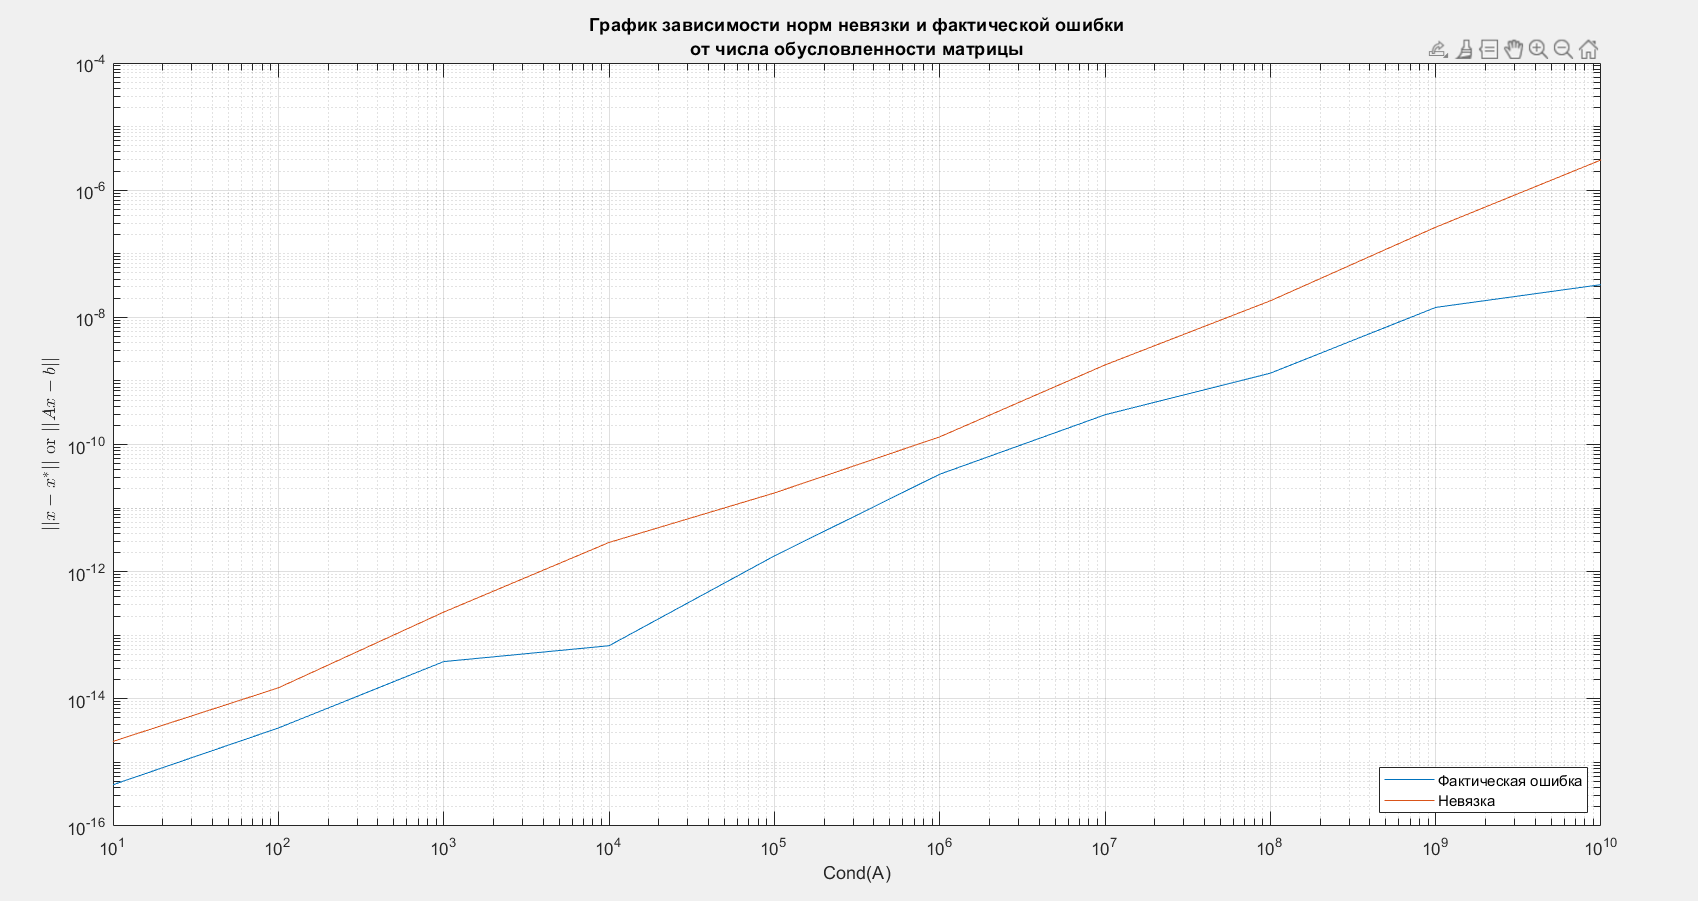
\includegraphics[scale = 0.4]{Точность}\\
	Результаты, полученные методом Холецкого, мы сравнили со специальной функцией "$\backslash$" в MATLAB. Из графика видно, что при хорошей обусловленности матрицы, погрешность решения выходит порядка $10^{-15}$, а при плохой обусловленности, например при cond(A) = $10^10$, погрешность возрастает до порядка $10^{-7}$.\\
	$\triangleright$ \underline{Возмущение:}\\
	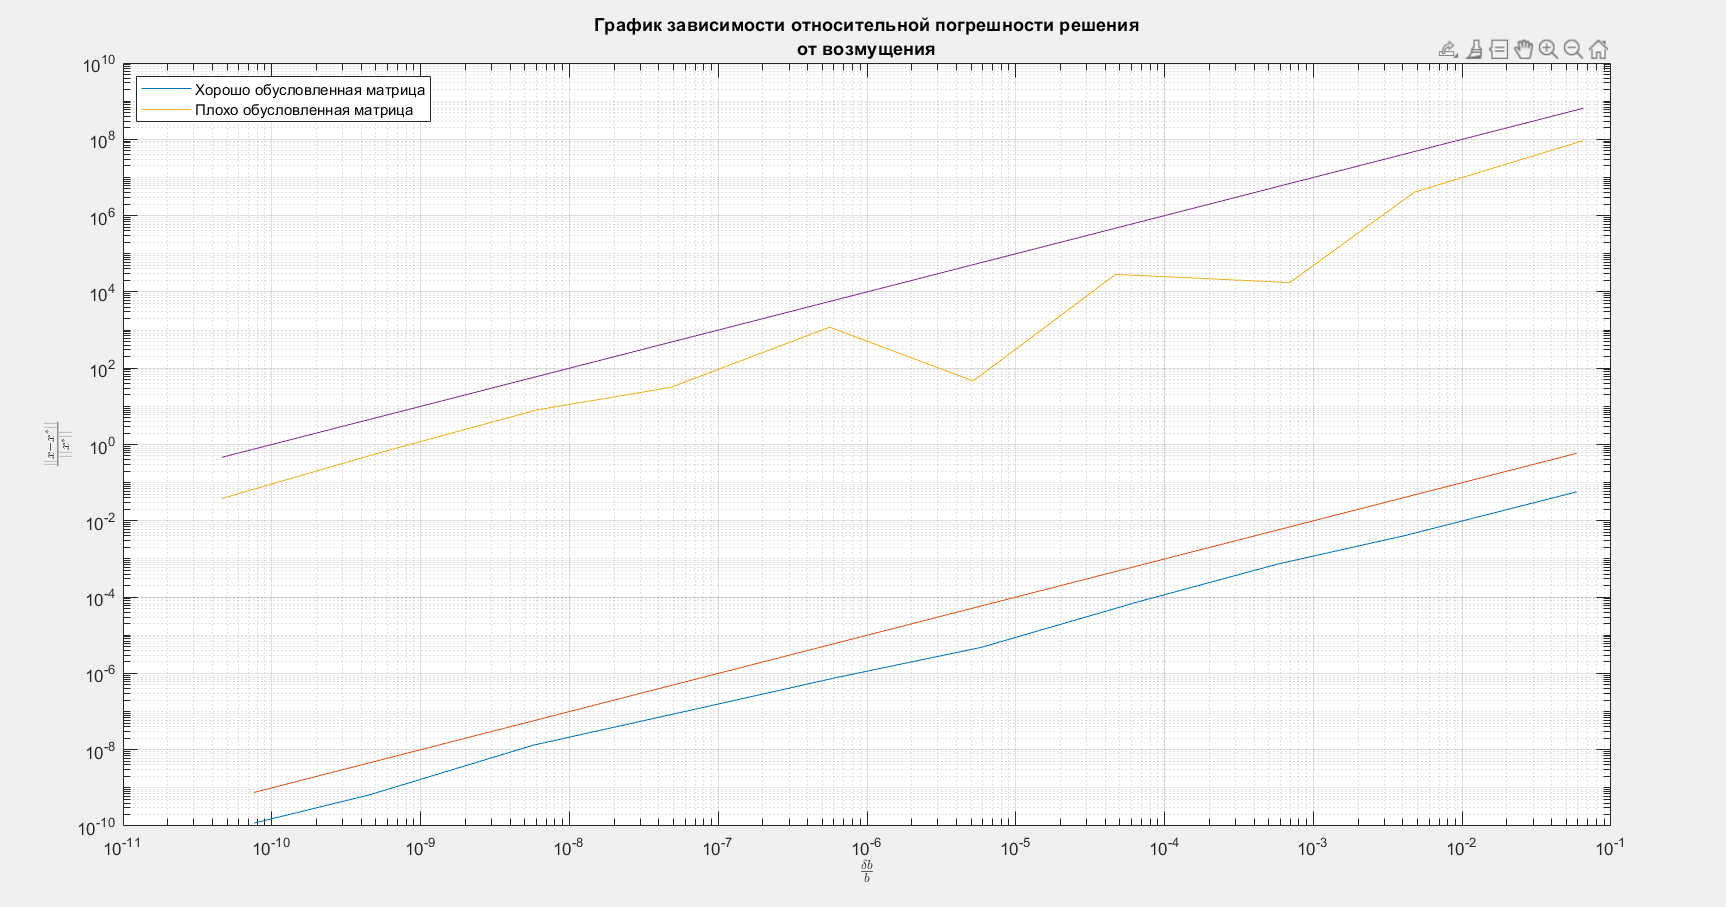
\includegraphics[scale = 0.394]{Возмущение}\\
	Из графика видно, что возмущение правой части оказывает большее влияние на плохо обусловленную матрицу, что и ожидалось. Так же выполняется неравенство $\frac{\delta x}{x} \leq cond(A)\frac{\delta b}{b}$\\
	\newpage
	$\triangleright$ \underline{Время выполнения:}\\
	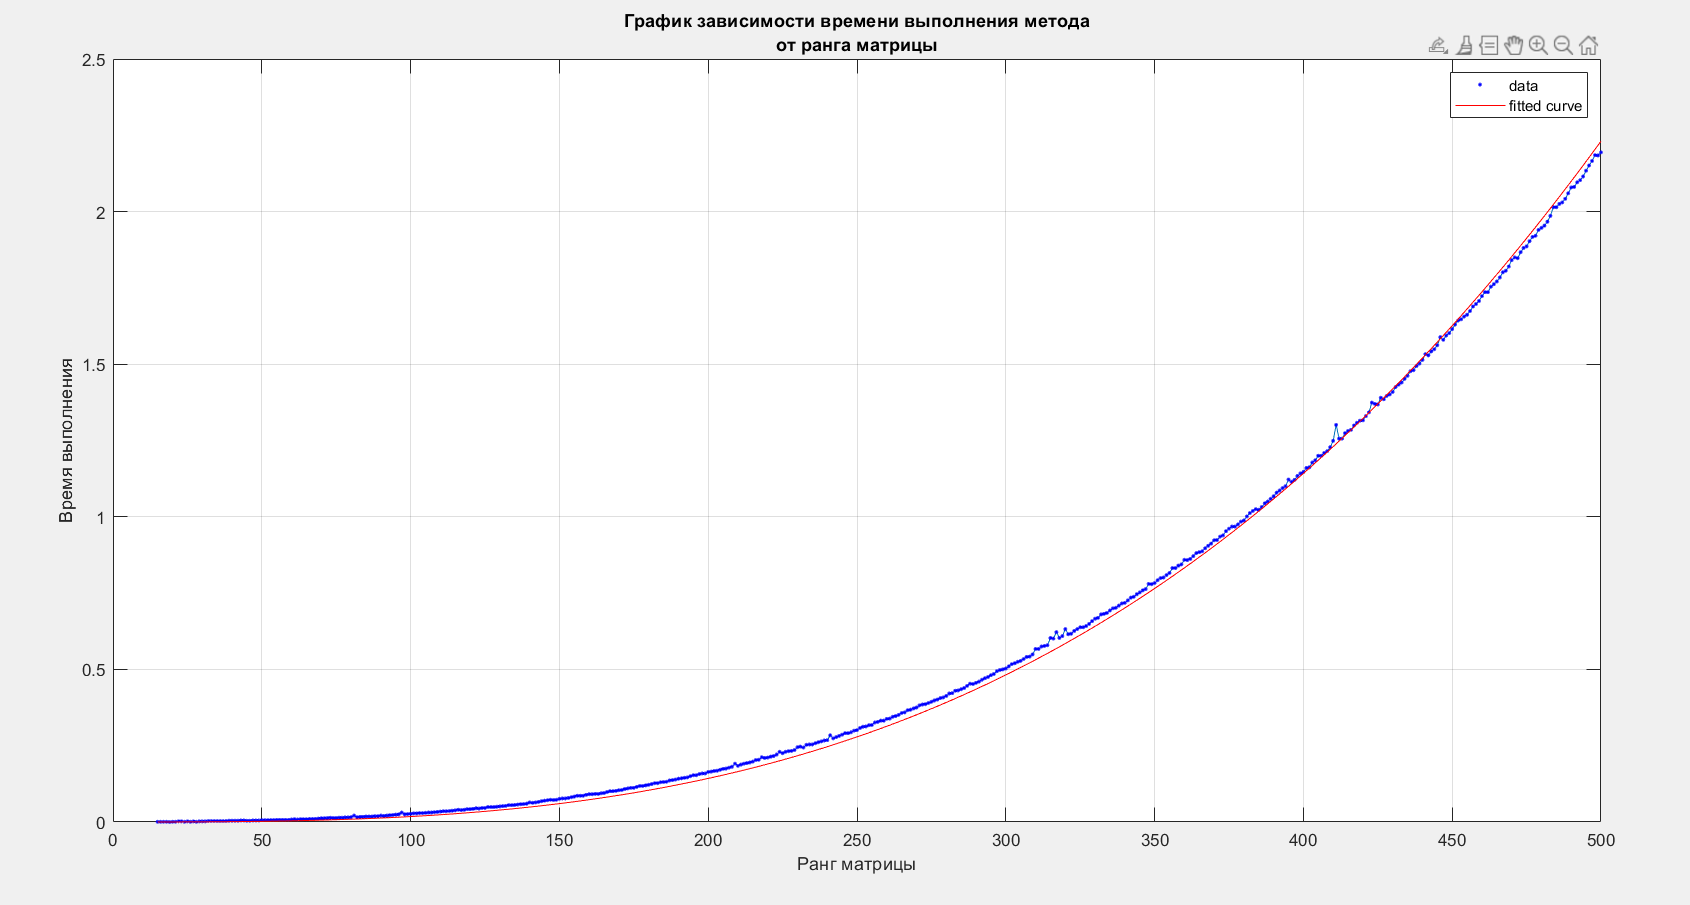
\includegraphics[scale = 0.4]{Время выполнения}\\
	Из графика поолучаем зависимость $\sim n^3$, что и ожидаемо, т.к. Вычислительная сложность метода порядка $\frac{n^3}{3}$.
	\begin{center} \textbf{Общие выводы:}\end{center}
	В данной лабораторной работе мы научились находить решения СЛАУ методом Холецкого, рассмотрели зависимость погрешности решения от числа обусловленности матрицы и от возмущения правой части системы уравнений. В обоих случаях, чем больше число обусловленности матрицы, тем труднее найти более точное решение. Так же определили время выполнения метода Холецкого.
\end{document}